\documentclass[12pt,a4paper]{article}
\usepackage[margin=1in]{geometry}
\usepackage{amsmath,booktabs,hyperref,enumitem,xcolor,listings,tikz}
\usetikzlibrary{positioning,arrows.meta}
\lstset{language=Python,basicstyle=\ttfamily\small,keywordstyle=\color{blue},commentstyle=\color{gray},showstringspaces=false,breaklines=true,frame=single}
\title{Neural Network and Deep Learning\\Assignment Question 4}
\author{}\date{}
\begin{document}\maketitle
\section*{4. Transfer Learning}
Transfer learning reuses knowledge learned for a source task to solve a related target task. Instead of learning edges, textures, and object parts from random initialisation, a target model starts from a network trained on a large dataset such as ImageNet. The early layers usually learn general visual features; later layers are more task-specific.

\begin{center}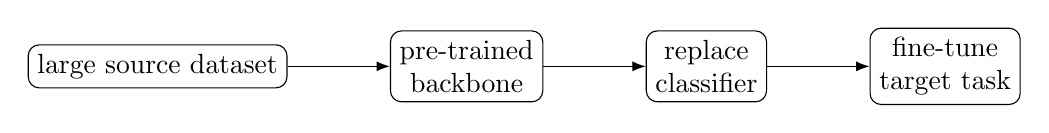
\begin{tikzpicture}[node distance=1.3cm,>=Latex, every node/.style={draw,rounded corners,align=center}]
\node (a){large source dataset};\node[right=of a](b){pre-trained\\backbone};\node[right=of b](c){replace\\classifier};\node[right=of c](d){fine-tune\\target task};
\draw[->](a)--(b);\draw[->](b)--(c);\draw[->](c)--(d);
\end{tikzpicture}\end{center}

Advantages are lower data requirements, shorter training time, better accuracy, and useful representations for small datasets. Risks include negative transfer when the source and target domains differ, inherited bias, inappropriate preprocessing, and leakage if test data influences fine-tuning. The target validation set must still guide decisions.

\subsection*{Feature extraction and fine-tuning}
In feature extraction, the pre-trained backbone is frozen and only a new classifier is trained. This is inexpensive and is a good first baseline. In fine-tuning, some upper backbone layers are unfrozen and trained with a very small learning rate after the new head has learned. Freezing the lower layers preserves general features and limits overfitting.
\begin{center}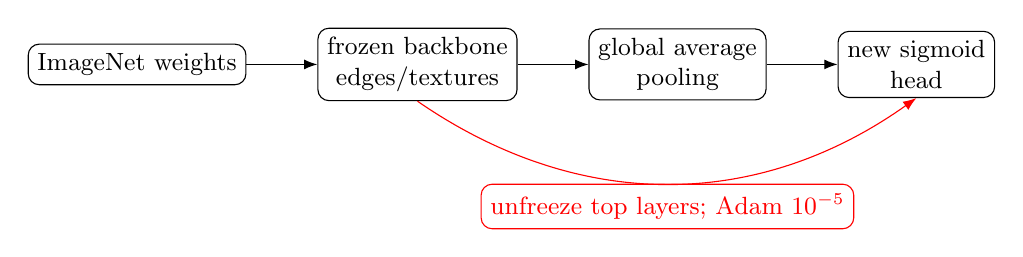
\begin{tikzpicture}[node distance=9mm,>=Latex, every node/.style={draw,rounded corners,align=center,font=\small}]
\node(a){ImageNet weights};\node[right=of a](b){frozen backbone\\edges/textures};\node[right=of b](c){global average\\pooling};\node[right=of c](d){new sigmoid\\head};\draw[->](a)--(b);\draw[->](b)--(c);\draw[->](c)--(d);\draw[red,->](b.south)to[bend right=35]node[below]{unfreeze top layers; Adam $10^{-5}$}(d.south);
\end{tikzpicture}\end{center}
For small, similar target data, freeze most layers. For larger or dissimilar data, unfreeze upper layers gradually. Negative transfer, domain shift, and catastrophic forgetting remain risks.

\subsection*{Python demonstration: cats versus dogs}
The directory \texttt{data/} is assumed to contain \texttt{cats/} and \texttt{dogs/} subdirectories. The program uses a pre-trained MobileNetV2 because it is small enough for an ordinary computer. It first trains a new two-class head, then optionally fine-tunes the final layers.
\begin{lstlisting}
import tensorflow as tf
from tensorflow.keras import layers
from tensorflow.keras.applications import MobileNetV2
from tensorflow.keras.applications.mobilenet_v2 import preprocess_input

train = tf.keras.utils.image_dataset_from_directory(
    "data", validation_split=.2, subset="training", seed=42,
    image_size=(160, 160), batch_size=32)
valid = tf.keras.utils.image_dataset_from_directory(
    "data", validation_split=.2, subset="validation", seed=42,
    image_size=(160, 160), batch_size=32)

base = MobileNetV2(include_top=False, weights="imagenet",
                   input_shape=(160, 160, 3))
base.trainable = False
inputs = tf.keras.Input((160, 160, 3))
x = preprocess_input(inputs)
x = base(x, training=False)
x = layers.GlobalAveragePooling2D()(x)
x = layers.Dropout(.2)(x)
outputs = layers.Dense(1, activation="sigmoid")(x)
model = tf.keras.Model(inputs, outputs)
model.compile("adam", "binary_crossentropy", metrics=["accuracy"])
model.fit(train, validation_data=valid, epochs=5)
print(model.evaluate(valid, verbose=0))

# Optional fine-tuning after the frozen-head stage has converged.
base.trainable = True
for layer in base.layers[:-20]:
    layer.trainable = False
model.compile(tf.keras.optimizers.Adam(1e-5),
              "binary_crossentropy", metrics=["accuracy"])
model.fit(train, validation_data=valid, epochs=3)
\end{lstlisting}
\texttt{image\_dataset\_from\_directory} infers labels from folder names and creates reproducible training and validation subsets. MobileNetV2's ImageNet weights are the source knowledge. \texttt{include\_top=False} removes its original 1000-class head. Global average pooling removes the spatial dimensions without a large flattening layer; dropout regularises the new classifier. \texttt{base.trainable=False} makes feature extraction cheap. When fine-tuning, only the last twenty layers adapt, and the learning rate is reduced by 100 times to avoid destroying useful features. Batch-normalisation layers are kept in inference mode by \texttt{training=False} while the backbone is called.

\paragraph{Representative output and interpretation.}
\begin{verbatim}
Epoch 5/5 - accuracy: 0.962 - val_accuracy: 0.928
[0.19, 0.928]
fine-tuning: val_accuracy 0.945
\end{verbatim}
The first value from \texttt{evaluate} is loss and the second is accuracy. Fine-tuning may improve validation accuracy, but it can also reduce it if the dataset is too small or the domains differ. The result must therefore be compared with the frozen baseline, not assumed in advance.
\end{document}